\documentclass[a4paper,9pt]{extarticle}

%=========================================================
% PACKAGES
%=========================================================

\usepackage[
a4paper,
top=1.8cm,
bottom=1.5cm,
footskip=7mm,
left=1cm,
right=1cm,
headheight=14pt,
headsep=5mm
]{geometry}

\usepackage[T1]{fontenc}
\usepackage[utf8]{inputenc}
\usepackage[french]{babel}

\usepackage[sfdefault]{FiraSans}
\renewcommand{\familydefault}{\sfdefault}

\usepackage{multicol}
\setlength{\columnsep}{0.7cm}

\usepackage{amsmath,amssymb}
\usepackage{titlesec}
\usepackage{enumitem}

\usepackage{tcolorbox}
\tcbuselibrary{skins,breakable}

\usepackage{xcolor}
\usepackage{graphicx}
\usepackage{float}
\usepackage{tikz}

\usepackage{fancyhdr}
\usepackage[hidelinks]{hyperref}


%=========================================================
% PAGE SETTINGS
%=========================================================

\setlength{\parindent}{0pt}
\setlength{\parskip}{1.5pt}

\setlength{\abovedisplayskip}{4pt}
\setlength{\belowdisplayskip}{4pt}

\setlist[itemize]{
leftmargin=*,
itemsep=1pt,
topsep=1pt
}


%=========================================================
% COLORS
%=========================================================

\definecolor{Blue}{HTML}{E3F0FF}
\definecolor{Green}{HTML}{E3F7EA}
\definecolor{Pink}{HTML}{FFE5ED}
\definecolor{Orange}{HTML}{FFF0DC}
\definecolor{Purple}{HTML}{EEE7FF}
\definecolor{Yellow}{HTML}{FFFADB}

\definecolor{BlueTitle}{HTML}{285B8F}
\definecolor{GreenTitle}{HTML}{287052}
\definecolor{PinkTitle}{HTML}{A84063}
\definecolor{OrangeTitle}{HTML}{A96500}
\definecolor{PurpleTitle}{HTML}{6245A5}


%=========================================================
% HEADER
%=========================================================

\pagestyle{fancy}
\fancyhf{}

\fancyhead[L]{\small\textbf{Electronique I}}
\fancyhead[C]{\small Diagrammes de Bode}
\fancyhead[R]{\small Week 06 -- 12-18/10/2026}

\fancyfoot[C]{\small\href{https://github.com/AlphaXT38G/notes_ba5}{github.com/AlphaXT38G/notes\_ba5}}
\fancyfoot[R]{\small \thepage}

\renewcommand{\headrulewidth}{0.4pt}


%=========================================================
% TITLES
%=========================================================

\titleformat{\section}
{\large\bfseries\color{BlueTitle}}
{}{0pt}{}

\titlespacing{\section}
{0pt}{6pt}{3pt}


%=========================================================
% SEPARATOR
%=========================================================

\newcommand{\separator}{
\vspace{2pt}
\hrule
\vspace{3pt}
}


%=========================================================
% BOXES
%=========================================================

% DEFINITION - blue

\newtcolorbox{definition}{
enhanced,
breakable,
colback=Blue,
colframe=BlueTitle,
boxrule=0.7pt,
arc=0mm,
title=\textbf{Definition},
fonttitle=\bfseries
}


% IMPORTANT - pink

\newtcolorbox{important}{
enhanced,
breakable,
colback=Pink,
colframe=PinkTitle,
boxrule=0.7pt,
arc=0mm,
title=\textbf{Key idea},
fonttitle=\bfseries
}


% FORMULAS - green

% optional argument: extra options, e.g. [unbreakable] for a box that multicols misplaces
\newtcolorbox{formula}[1][]{
enhanced,
breakable,
colback=Green,
colframe=GreenTitle,
boxrule=0.7pt,
arc=0mm,
title=\textbf{Key formulas},
fonttitle=\bfseries,
#1
}


% WARNING - orange

\newtcolorbox{warning}{
enhanced,
breakable,
colback=Orange,
colframe=OrangeTitle,
boxrule=0.7pt,
arc=0mm,
title=\textbf{Warning},
fonttitle=\bfseries
}


% EXAMPLE - purple

\newtcolorbox{example}{
enhanced,
breakable,
colback=Purple,
colframe=PurpleTitle,
boxrule=0.7pt,
arc=0mm,
title=\textbf{Example},
fonttitle=\bfseries
}


% SUMMARY - yellow

\newtcolorbox{summary}{
enhanced,
breakable,
colback=Yellow,
colframe=OrangeTitle,
boxrule=0.7pt,
arc=0mm,
title=\textbf{Summary},
fonttitle=\bfseries
}


% a box only breaks once it has a few lines on this column: no lone title at the bottom
\tcbset{lines before break=8}


%=========================================================
% DOCUMENT
%=========================================================

\begin{document}

\thispagestyle{fancy}

\footnotesize

\begin{multicols}{2}


%=========================================================
\section{Introduction : où on en est}


\begin{center}

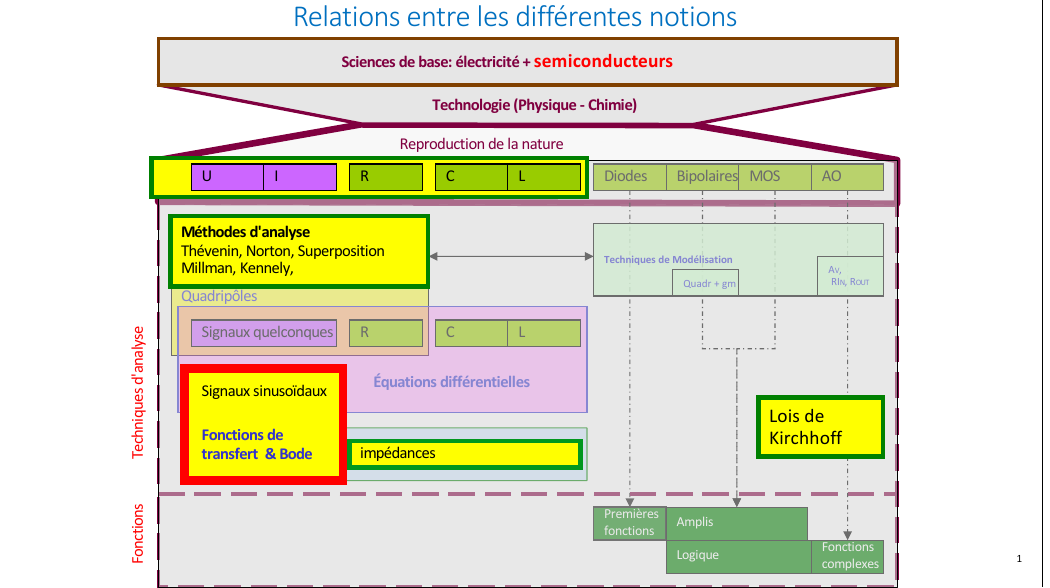
\includegraphics[
width=1.0\linewidth
]{../images/week06_01.png}

\end{center}

Après la notion d'impédances complexes, assimilables à des résistances, on développe un outil d'analyse \textbf{graphique} du comportement de circuits combinant plusieurs impédances (résistances et condensateurs en particulier). Chaque circuit met en évidence une expression appelée \textbf{fonction de transfert}. Son analyse est divisée en deux parties :

\begin{itemize}

\item le \textbf{diagramme de Bode du module} : le rapport entre l'amplitude du signal de sortie et celle du signal d'entrée, selon la fréquence ;

\item le \textbf{diagramme de Bode en phase} : le déphasage entre le signal de sortie et celui d'entrée, selon la fréquence.

\end{itemize}


\begin{center}

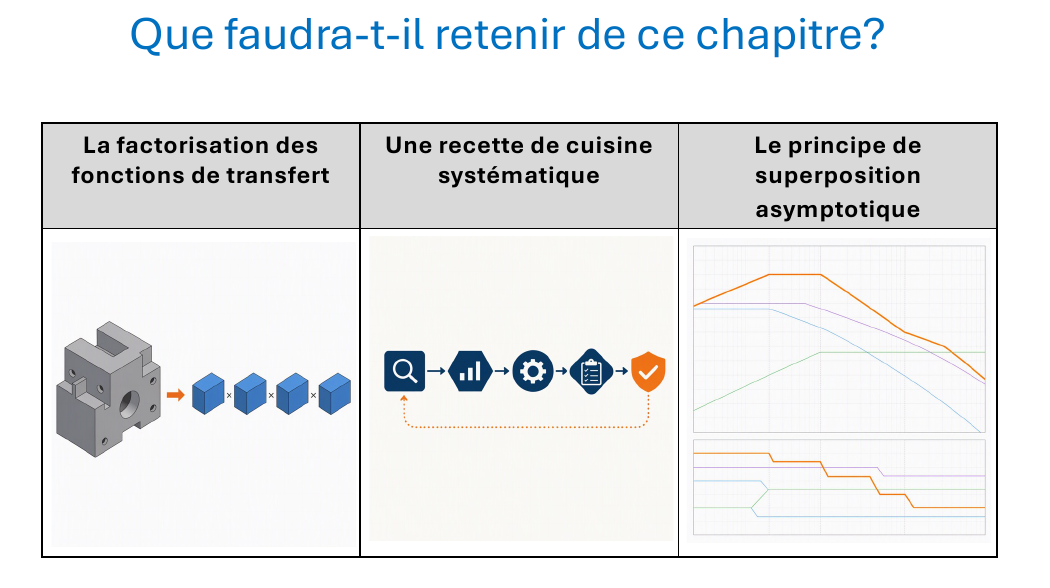
\includegraphics[
width=1.0\linewidth
]{../images/week06_02.png}

\end{center}


\begin{summary}

\textbf{Que faudra-t-il retenir de ce chapitre ?}

\begin{enumerate}[leftmargin=*,itemsep=1pt,topsep=1pt]

\item \textbf{La factorisation des fonctions :} selon la taille des circuits, les fonctions de transfert peuvent devenir imposantes et délicates à traiter. Le premier effort sera de les factoriser en un produit de \textbf{termes fondamentaux du premier ordre}, comme on décompose un polynôme de degré $N$.

\item \textbf{Une recette de cuisine systématique :} évaluer les comportements physiques du circuit aux limites ($\omega \to 0$ et $\omega \to \infty$), puis, à partir des impédances, écrire la fonction de transfert sous sa \textbf{forme canonique}, vérifier sa cohérence mathématique, et enfin tracer les diagrammes de Bode (module et argument).

\item \textbf{Le principe de superposition asymptotique :} tracer un diagramme de Bode global est un \og jeu \fg{} de construction. On reporte sur le graphique le dessin de chaque terme élémentaire, indépendamment des autres. Chaque dessin est toujours sous forme de \textbf{droites asymptotiques}. Il ne reste plus qu'à additionner graphiquement ces droites, intervalle par intervalle, pour obtenir la résultante finale.

\end{enumerate}

\end{summary}


\begin{important}

\textbf{En très simple : de quoi parle ce chapitre ?}

La semaine dernière, on a obtenu des fonctions de transfert comme $\underline{H} = \frac{1}{1 + j\omega RC}$ : elles disent ce que le circuit fait à un sinus (le rétrécit et le décale), selon sa fréquence. Mais une formule, ça ne se \og voit \fg{} pas.

\vspace{3pt}

Le \textbf{diagramme de Bode}, c'est le \textbf{dessin} de cette fonction : deux graphes l'un sous l'autre,

\begin{itemize}

\item en haut : de combien le sinus est \textbf{agrandi ou rétréci}, pour chaque fréquence ;

\item en bas : de combien il est \textbf{décalé}, pour chaque fréquence.

\end{itemize}

D'un coup d'œil, on voit si le circuit laisse passer les graves, les aigus, ou une bande au milieu.

\vspace{3pt}

\textbf{L'astuce du chapitre :} on découpe la fonction en petits morceaux tout simples, on dessine chaque morceau avec des \textbf{lignes droites}, et on additionne les dessins. Comme des Lego.

\end{important}


%=========================================================
\section{Objectifs de la séance : la forme canonique}


\begin{center}

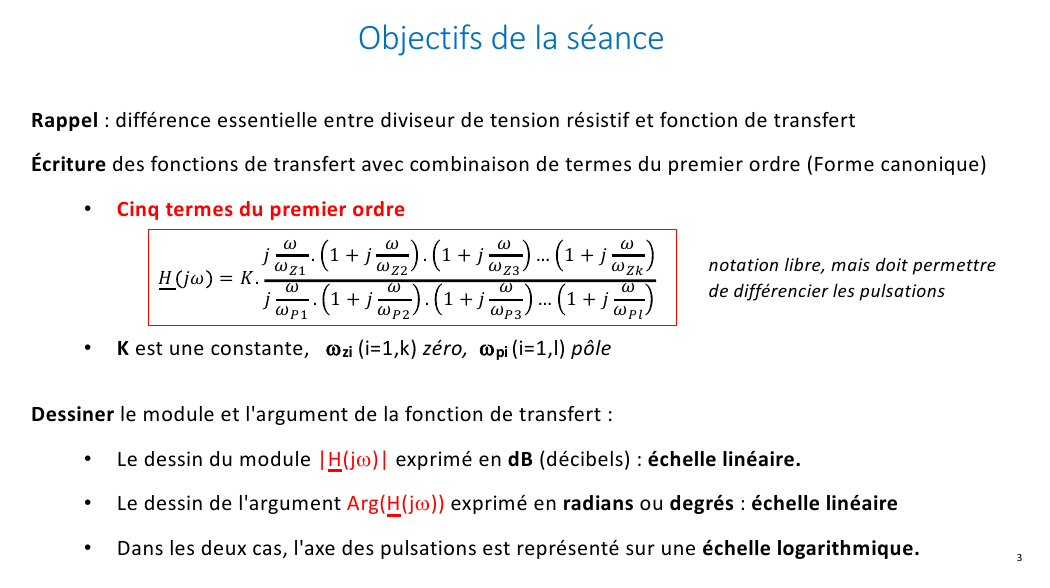
\includegraphics[
width=1.0\linewidth
]{../images/week06_03.png}

\end{center}

\begin{itemize}

\item \textbf{Rappel :} différence essentielle entre diviseur de tension résistif et fonction de transfert.

\item \textbf{Écriture} des fonctions de transfert avec une combinaison de termes du premier ordre (forme canonique).

\item \textbf{Dessiner} le module et l'argument de la fonction de transfert.

\end{itemize}


\begin{formula}

Cinq termes du premier ordre (forme canonique) :

\[
\underline{H}(j\omega) = K \cdot \frac{j\frac{\omega}{\omega_{Z1}} \cdot \left(1 + j\frac{\omega}{\omega_{Z2}}\right)\left(1 + j\frac{\omega}{\omega_{Z3}}\right)\cdots\left(1 + j\frac{\omega}{\omega_{Zk}}\right)}{j\frac{\omega}{\omega_{P1}} \cdot \left(1 + j\frac{\omega}{\omega_{P2}}\right)\left(1 + j\frac{\omega}{\omega_{P3}}\right)\cdots\left(1 + j\frac{\omega}{\omega_{Pl}}\right)}
\]

(notation libre, mais elle doit permettre de différencier les pulsations).

où :

\begin{itemize}

\item $K$ : une constante [sans unité] ;

\item $\omega_{Zi}$ ($i = 1, \dots, k$) : pulsations des \textbf{zéros} (dans le numérateur) [rad/s] ;

\item $\omega_{Pi}$ ($i = 1, \dots, l$) : pulsations des \textbf{pôles} (dans le dénominateur) [rad/s] ;

\item $\omega$ : pulsation du signal [rad/s].

\end{itemize}

\end{formula}

\begin{itemize}

\item Le dessin du module $|\underline{H}(j\omega)|$ est exprimé en \textbf{dB} (décibels) : échelle linéaire.

\item Le dessin de l'argument $\operatorname{Arg}(\underline{H}(j\omega))$ est exprimé en \textbf{radians} ou \textbf{degrés} : échelle linéaire.

\item Dans les deux cas, l'axe des pulsations est représenté sur une \textbf{échelle logarithmique}.

\end{itemize}

Les fonctions de transfert sont souvent des produits de termes de base simples, dits du premier ordre, répartis en 5 catégories. Dans ces termes apparaissent des \textbf{pulsations caractéristiques} : on parle de \textbf{pôle} quand la pulsation est dans un terme du dénominateur, et de \textbf{zéro} quand elle est dans un terme du numérateur. Ces termes de base sont individuellement très faciles à dessiner (des dessins linéaires par intervalles) ; en les combinant, il est très simple de dessiner le module et l'argument de la fonction complète.


\begin{important}

\textbf{En très simple : les 5 briques}

Toute fonction de transfert de ce cours se construit avec seulement \textbf{5 briques} :

\begin{enumerate}[leftmargin=*,itemsep=1pt,topsep=1pt]

\item $K$ : un simple nombre ;

\item $j\frac{\omega}{\omega_Z}$ : un \og $j\omega$ tout seul \fg{} en haut ;

\item $1 + j\frac{\omega}{\omega_Z}$ : un \og 1 plus $j\omega$ \fg{} en haut ;

\item $\frac{1}{j\omega/\omega_P}$ : un \og $j\omega$ tout seul \fg{} en bas ;

\item $\frac{1}{1 + j\omega/\omega_P}$ : un \og 1 plus $j\omega$ \fg{} en bas.

\end{enumerate}

La \textbf{forme canonique}, c'est réécrire la fonction pour qu'elle ne soit qu'une multiplication de ces briques. Chaque brique a sa propre \og fréquence spéciale \fg{} ($\omega_Z$ ou $\omega_P$), là où elle change de comportement.

\vspace{3pt}

\textbf{Zéro ou pôle ?} Un zéro est en haut de la fraction, un pôle en bas. Le nom vient des maths : en haut, la brique peut annuler la fraction (zéro) ; en bas, elle peut la faire exploser (pôle).

\vspace{3pt}

\textbf{Échelle logarithmique} : sur l'axe des fréquences, les graduations ne vont pas $1, 2, 3, 4$ mais $1, 10, 100, 1000$ : chaque pas multiplie par 10. Ça permet de voir sur un seul dessin des fréquences très petites et très grandes.

\end{important}


%=========================================================
\section{Rappel : différence essentielle entre $R$ et $\underline{Z}$}


\begin{center}

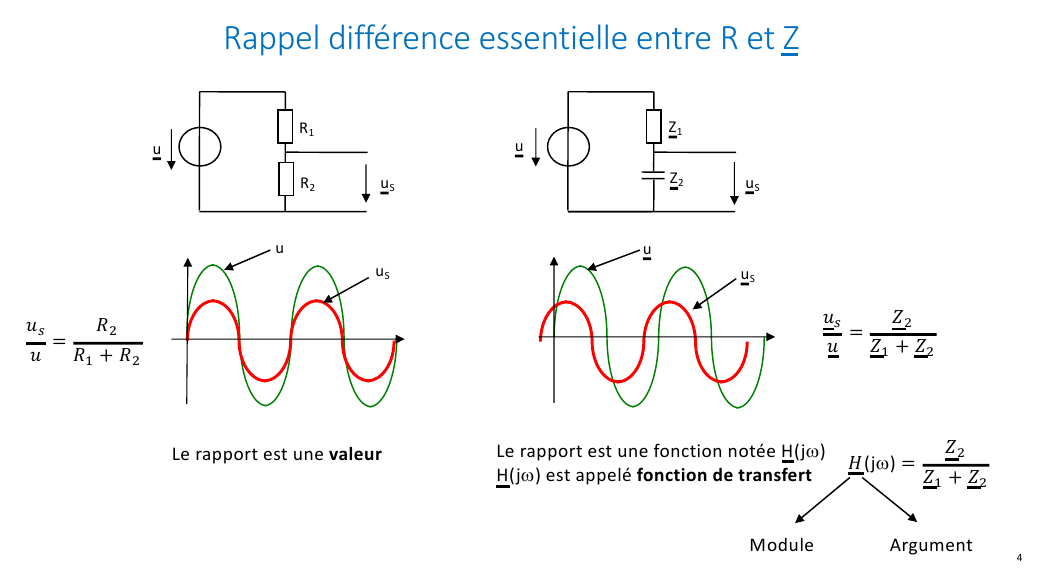
\includegraphics[
width=1.0\linewidth
]{../images/week06_04.png}

\end{center}


\begin{formula}

Avec deux résistances, le rapport est une \textbf{valeur} :

\[
\frac{u_S}{u} = \frac{R_2}{R_1 + R_2}
\]

Avec des impédances, le rapport est une \textbf{fonction}, notée $\underline{H}(j\omega)$ et appelée \textbf{fonction de transfert} (avec un module et un argument) :

\[
\underline{H}(j\omega) = \frac{\underline{u}_S}{\underline{u}} = \frac{\underline{Z}_2}{\underline{Z}_1 + \underline{Z}_2}
\]

où :

\begin{itemize}

\item $u$, $\underline{u}$ : tension d'entrée [V] ; $u_S$, $\underline{u}_S$ : tension de sortie [V] ;

\item $R_1$, $R_2$ : résistances [$\Omega$] ; $\underline{Z}_1$, $\underline{Z}_2$ : impédances [$\Omega$] ;

\item $\underline{H}(j\omega)$ : fonction de transfert [sans unité].

\end{itemize}

\end{formula}

La fonction de transfert la plus simple est le diviseur résistif, avec deux résistances. Quelle que soit la fréquence, le rapport entre l'amplitude de sortie et celle d'entrée est constant, et il n'y a pas de décalage entre les deux signaux. Si l'une des résistances est remplacée par un condensateur, l'amplitude varie avec la fréquence, de même que le décalage.


\begin{important}

\textbf{En très simple : les deux dessins}

\textbf{À gauche (deux résistances)} : la sortie (rouge) est un sinus plus petit que l'entrée (vert), mais \textbf{parfaitement aligné} : mêmes sommets au même moment. Et ce rapport de taille est le même pour toutes les fréquences : c'est juste un nombre, par exemple $0.5$.

\vspace{3pt}

\textbf{À droite (résistance et condensateur)} : la sortie est plus petite \textbf{et décalée} (ses sommets arrivent plus tôt ou plus tard). Et la taille comme le décalage changent selon la fréquence. Ce n'est plus un nombre, c'est une fonction de la fréquence : $\underline{H}(j\omega)$.

\vspace{3pt}

C'est pour dessiner cette fonction qu'on a besoin des diagrammes de Bode.

\end{important}


%=========================================================
\section{Produits de termes de base et décibels}


\begin{center}

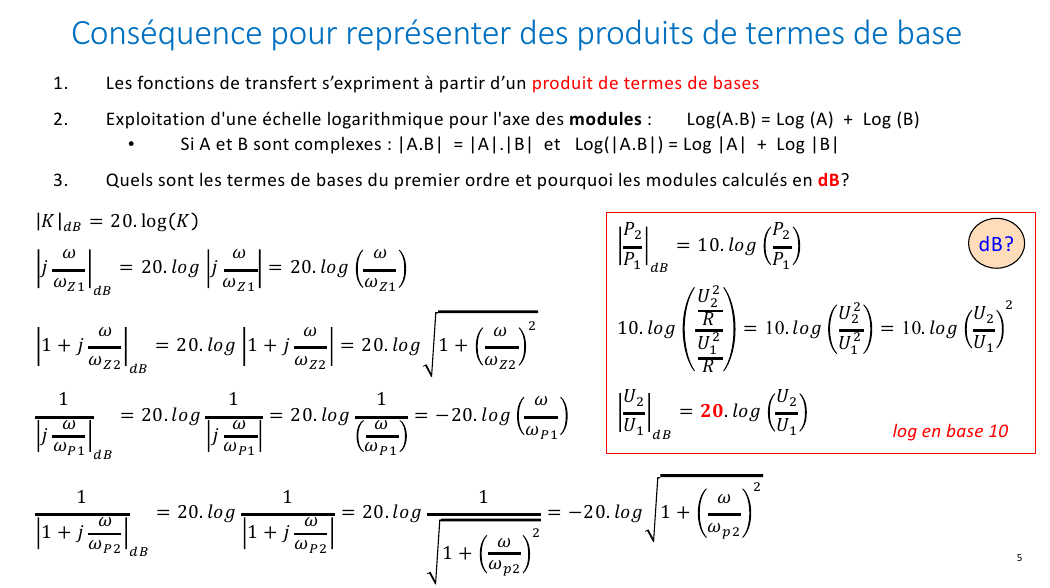
\includegraphics[
width=1.0\linewidth
]{../images/week06_05.png}

\end{center}

\begin{enumerate}[leftmargin=*,itemsep=1pt,topsep=1pt]

\item Les fonctions de transfert s'expriment à partir d'un \textbf{produit de termes de base}.

\item On exploite une échelle logarithmique pour l'axe des modules : $\log(A\cdot B) = \log(A) + \log(B)$. Si $A$ et $B$ sont complexes : $|A\cdot B| = |A|\cdot|B|$ et $\log(|A\cdot B|) = \log|A| + \log|B|$.

\item Quels sont les termes de base du premier ordre, et pourquoi les modules sont-ils calculés en dB ?

\end{enumerate}


\begin{formula}

Le décibel (log en base 10), défini pour un rapport de puissances :

\[
\left|\frac{P_2}{P_1}\right|_{dB} = 10\log\left(\frac{P_2}{P_1}\right)
\]
\[
10\log\left(\frac{U_2^2/R}{U_1^2/R}\right) = 10\log\left(\frac{U_2^2}{U_1^2}\right) = 10\log\left(\frac{U_2}{U_1}\right)^2
\;\Rightarrow\;
\boxed{\left|\frac{U_2}{U_1}\right|_{dB} = 20\log\left(\frac{U_2}{U_1}\right)}
\]

Les modules des 5 termes de base, en dB :

\[
|K|_{dB} = 20\log(K)
\]
\[
\left|j\frac{\omega}{\omega_{Z1}}\right|_{dB} = 20\log\left(\frac{\omega}{\omega_{Z1}}\right)
\]
\[
\left|1 + j\frac{\omega}{\omega_{Z2}}\right|_{dB} = 20\log\sqrt{1 + \left(\frac{\omega}{\omega_{Z2}}\right)^2}
\]
\[
\left|\frac{1}{j\frac{\omega}{\omega_{P1}}}\right|_{dB} = 20\log\frac{1}{\left(\frac{\omega}{\omega_{P1}}\right)} = -20\log\left(\frac{\omega}{\omega_{P1}}\right)
\]
\[
\left|\frac{1}{1 + j\frac{\omega}{\omega_{P2}}}\right|_{dB} = 20\log\frac{1}{\sqrt{1 + \left(\frac{\omega}{\omega_{P2}}\right)^2}} = -20\log\sqrt{1 + \left(\frac{\omega}{\omega_{P2}}\right)^2}
\]

où :

\begin{itemize}

\item $P_1$, $P_2$ : puissances [W] ; $U_1$, $U_2$ : tensions [V] ; $R$ : résistance [$\Omega$] ;

\item $|\cdot|_{dB}$ : module exprimé en décibels [dB] ; $\log$ : logarithme en base 10 ;

\item $K$ : constante ; $\omega_{Z}$, $\omega_{P}$ : pulsations caractéristiques [rad/s] ; $\omega$ [rad/s].

\end{itemize}

\end{formula}

Le module d'un produit est égal au produit des modules : via le logarithme, il suffit de \textbf{sommer} les valeurs en dB des différents modules. Le dB vient d'un rapport de puissances, $10\log(P_2/P_1)$ (comme en acoustique). Pour des tensions, on utilise $20\log(U_2/U_1)$ : comme $P = U^2/R$, extraire le carré du log revient à multiplier le log par 2 ($\log x^2 = 2\log x$), d'où le facteur 20 au lieu de 10.


\begin{definition}

\textbf{Décibel (dB)}

Une façon d'exprimer un rapport (ici sortie/entrée) avec un logarithme : $20\log(\text{rapport})$ pour des tensions.

\end{definition}


\begin{important}

\textbf{En très simple : pourquoi les décibels ?}

Le logarithme a un super-pouvoir : il \textbf{transforme les multiplications en additions}. Notre fonction de transfert est une multiplication de briques ; en dB, elle devient une \textbf{addition} de briques. Et additionner des dessins, c'est facile : on empile les courbes.

\vspace{3pt}

\textbf{Les chiffres à connaître} (le rapport de tensions $\rightarrow$ en dB) :

\begin{itemize}

\item $\times 1$ $\rightarrow$ $0\,\text{dB}$ (rien ne change) ;

\item $\times 10$ $\rightarrow$ $+20\,\text{dB}$ ; $\times 0.1$ $\rightarrow$ $-20\,\text{dB}$ ;

\item $\times 2$ $\rightarrow$ $+6\,\text{dB}$ ; $\times 0.5$ $\rightarrow$ $-6\,\text{dB}$ ;

\item $\times \frac{1}{\sqrt{2}} \approx 0.707$ $\rightarrow$ $-3\,\text{dB}$.

\end{itemize}

Positif = le circuit \textbf{agrandit} le signal ; négatif = il le \textbf{rétrécit}.

\vspace{3pt}

\textbf{Pourquoi 20 et pas 10 ?} Le dB est fait pour les puissances ($10\log$). Une puissance, c'est une tension au carré ($U^2/R$), et le log d'un carré, c'est deux fois le log : $10 \times 2 = 20$.

\end{important}


%=========================================================
\section{L'exemple le plus simple : le filtre passe-bas}


\begin{center}

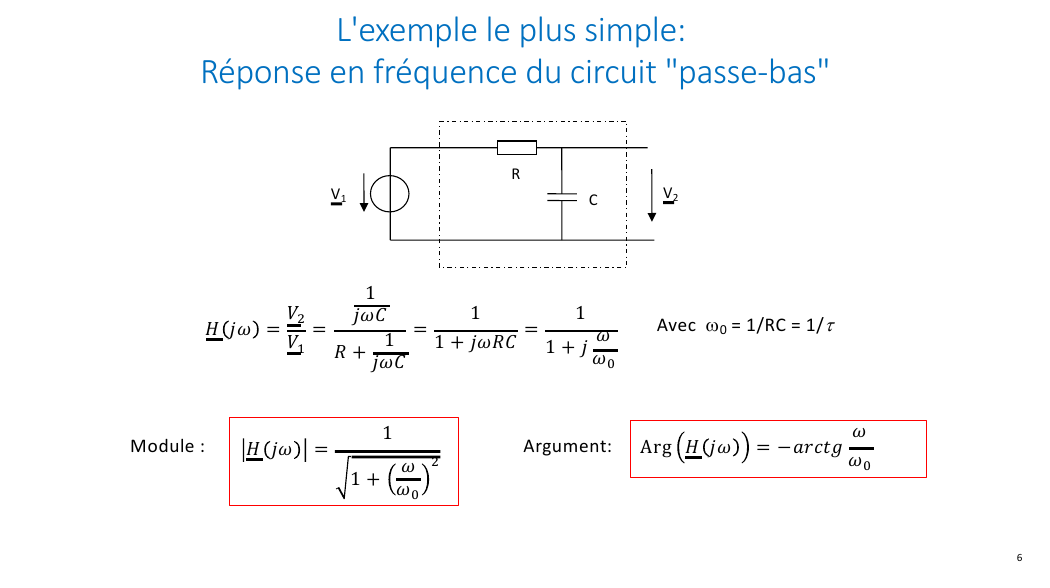
\includegraphics[
width=1.0\linewidth
]{../images/week06_06.png}

\end{center}


\begin{formula}

\[
\underline{H}(j\omega) = \frac{\underline{V}_2}{\underline{V}_1} = \frac{\frac{1}{j\omega C}}{R + \frac{1}{j\omega C}} = \frac{1}{1 + j\omega RC} = \frac{1}{1 + j\frac{\omega}{\omega_0}}
\quad\text{avec}\quad
\omega_0 = \frac{1}{RC} = \frac{1}{\tau}
\]

Module et argument :

\[
|\underline{H}(j\omega)| = \frac{1}{\sqrt{1 + \left(\frac{\omega}{\omega_0}\right)^2}}
\qquad
\operatorname{Arg}(\underline{H}(j\omega)) = -\operatorname{arctg}\frac{\omega}{\omega_0}
\]

où :

\begin{itemize}

\item $\underline{V}_1$ : tension d'entrée [V] ; $\underline{V}_2$ : tension de sortie, aux bornes de $C$ [V] ;

\item $R$ [$\Omega$] ; $C$ [F] ; $\tau = RC$ : constante de temps [s] ;

\item $\omega_0$ : pulsation caractéristique (de coupure) [rad/s].

\end{itemize}

\end{formula}

On illustre les échelles logarithmiques avec les filtres du cours précédent, le passe-bas et le passe-haut. Le produit $RC$ correspond à une pulsation particulièrement importante, la pulsation caractéristique $\omega_0 = 1/RC$. Pour dessiner ce comportement, la méthode la plus longue mais la plus sûre est de dessiner un grand nombre de points.


\begin{center}

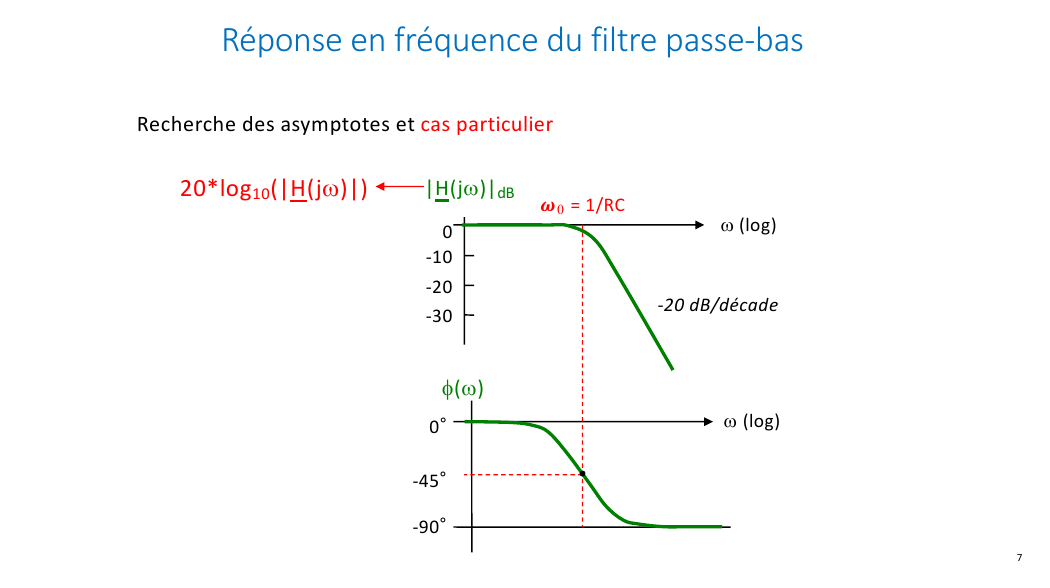
\includegraphics[
width=1.0\linewidth
]{../images/week06_07.png}

\end{center}

Recherche des asymptotes et cas particulier. Le module est tracé en $20\log_{10}(|\underline{H}(j\omega)|)$. Entre les très basses fréquences et la pulsation de coupure, l'évolution du module est très lente ; à partir de la pulsation de coupure, la pente s'accélère violemment ($-20\,\text{dB/décade}$). Pour l'argument, le déphasage est très faible en basses fréquences, s'accélère vers la pulsation de coupure et un peu au-delà, puis se stabilise à $-90°$. On travaillera plus simplement avec des courbes \textbf{asymptotiques} qui approximent correctement la réalité.


\begin{important}

\textbf{En très simple : lire le diagramme du passe-bas}

\textbf{En haut (le module en dB)} :

\begin{itemize}

\item à gauche (fréquences basses), la courbe est plate à $0\,\text{dB}$ : le signal passe sans être rétréci ;

\item à partir de $\omega_0$, elle plonge : $-20\,\text{dB}$ à chaque fois que la fréquence est multipliée par 10 (une \textbf{décade}). Le signal est divisé par 10 à chaque décade.

\end{itemize}

\textbf{En bas (la phase)} : elle part de $0°$ (pas de décalage), passe par $-45°$ pile à $\omega_0$, et finit à $-90°$ (décalage d'un quart de tour en retard).

\vspace{3pt}

\textbf{Pourquoi $\omega_0 = 1/RC$ ?} C'est là que $\frac{\omega}{\omega_0} = 1$ : la partie réelle ($1$) et la partie imaginaire ($\omega/\omega_0$) du dénominateur sont égales. Avant, le \og 1 \fg{} domine ; après, c'est le \og $j\omega/\omega_0$ \fg{}.

\end{important}


\begin{example}

$R = 1\,\text{k}\Omega$, $C = 1\,\mu\text{F}$ : $\omega_0 = 1000\,\text{rad/s}$.

\begin{itemize}

\item à $\omega = 1000$ : $|\underline{H}| = \frac{1}{\sqrt 2}$, soit $-3\,\text{dB}$, et $-45°$ ;

\item à $\omega = 10\,000$ : $|\underline{H}| \approx 0.1$, soit $-20\,\text{dB}$ ;

\item à $\omega = 100\,000$ : $|\underline{H}| \approx 0.01$, soit $-40\,\text{dB}$.

\end{itemize}

\end{example}


%=========================================================
\section{Approximation asymptotique}


\begin{center}

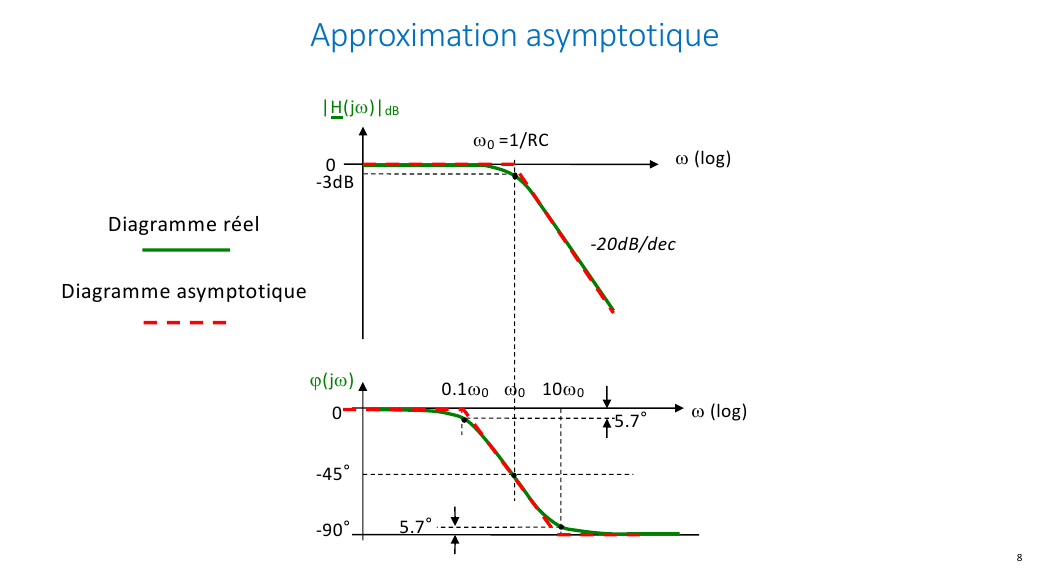
\includegraphics[
width=1.0\linewidth
]{../images/week06_08.png}

\end{center}

Diagramme réel (vert) et diagramme asymptotique (rouge pointillé).

\begin{itemize}

\item \textbf{Module :} deux asymptotes approximent correctement la courbe réelle. L'erreur maximale est obtenue à la pulsation caractéristique ; l'axe vertical étant en dB ($20\log$ du module), cette erreur représente $-3\,\text{dB}$.

\item \textbf{Argument :} trois asymptotes. Une horizontale pour les basses fréquences jusqu'à $0.1\,\omega_0$, une autre horizontale de $10\,\omega_0$ aux hautes fréquences, et les deux sont reliées par une pente de $\pi/2$ pour deux décades. À la pulsation caractéristique, le déphasage est de $-45°$. L'écart maximal ($5.7°$) est en $0.1\,\omega_0$ et $10\,\omega_0$.

\end{itemize}


\begin{formula}

\[
\text{Erreur du module en } \omega_0 : \ 20\log\frac{1}{\sqrt{2}} \approx -3\,\text{dB}
\qquad
\text{Erreur de phase en } 0.1\,\omega_0 : \ \operatorname{arctg}(0.1) \approx 5.7°
\]

où :

\begin{itemize}

\item $\omega_0$ : pulsation caractéristique [rad/s] ;

\item une \textbf{décade} : un intervalle où la pulsation est multipliée par 10.

\end{itemize}

\end{formula}


\begin{definition}

\textbf{Asymptote}

Une droite dont la vraie courbe se rapproche de plus en plus, loin du point spécial. Ici, on remplace la vraie courbe par quelques segments de droite.

\end{definition}


\begin{important}

\textbf{En très simple : on dessine avec une règle}

La vraie courbe est arrondie, pénible à tracer point par point. Mais loin de $\omega_0$, elle est presque parfaitement droite. Alors on la remplace par des \textbf{segments de droite} :

\begin{itemize}

\item \textbf{module} : une ligne plate à $0\,\text{dB}$ jusqu'à $\omega_0$, puis une ligne qui descend de $20\,\text{dB}$ par décade. C'est un \og coude \fg{} en $\omega_0$. La vraie courbe passe juste $3\,\text{dB}$ sous le coude ;

\item \textbf{phase} : plat à $0°$ jusqu'à $\omega_0/10$, plat à $-90°$ après $10\,\omega_0$, et une rampe droite entre les deux, qui passe par $-45°$ en $\omega_0$.

\end{itemize}

L'erreur est petite ($3\,\text{dB}$ et $5.7°$ au pire) et le dessin se fait en 30 secondes avec une règle.

\end{important}


%=========================================================
\section{Circuit RC passe-haut}


\begin{center}

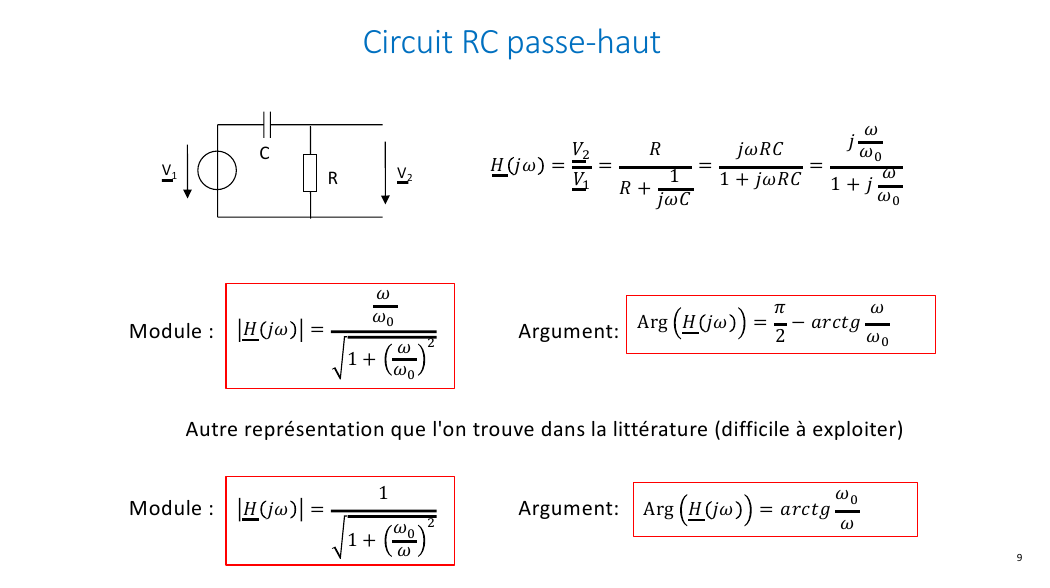
\includegraphics[
width=1.0\linewidth
]{../images/week06_09.png}

\end{center}


\begin{formula}

\[
\underline{H}(j\omega) = \frac{\underline{V}_2}{\underline{V}_1} = \frac{R}{R + \frac{1}{j\omega C}} = \frac{j\omega RC}{1 + j\omega RC} = \frac{j\frac{\omega}{\omega_0}}{1 + j\frac{\omega}{\omega_0}}
\]

\[
|\underline{H}(j\omega)| = \frac{\frac{\omega}{\omega_0}}{\sqrt{1 + \left(\frac{\omega}{\omega_0}\right)^2}}
\qquad
\operatorname{Arg}(\underline{H}(j\omega)) = \frac{\pi}{2} - \operatorname{arctg}\frac{\omega}{\omega_0}
\]

Autre représentation que l'on trouve dans la littérature (difficile à exploiter) :

\[
|\underline{H}(j\omega)| = \frac{1}{\sqrt{1 + \left(\frac{\omega_0}{\omega}\right)^2}}
\qquad
\operatorname{Arg}(\underline{H}(j\omega)) = \operatorname{arctg}\frac{\omega_0}{\omega}
\]

où $\omega_0 = 1/RC$ [rad/s] ; $\underline{V}_2$ : tension aux bornes de $R$ [V] ; les autres comme pour le passe-bas.

\end{formula}

Pour le filtre passe-haut, on obtient aussi une fonction de transfert et une pulsation caractéristique ($\omega_0 = 1/RC$), dont on déduit l'allure du module et de l'argument.


\begin{center}

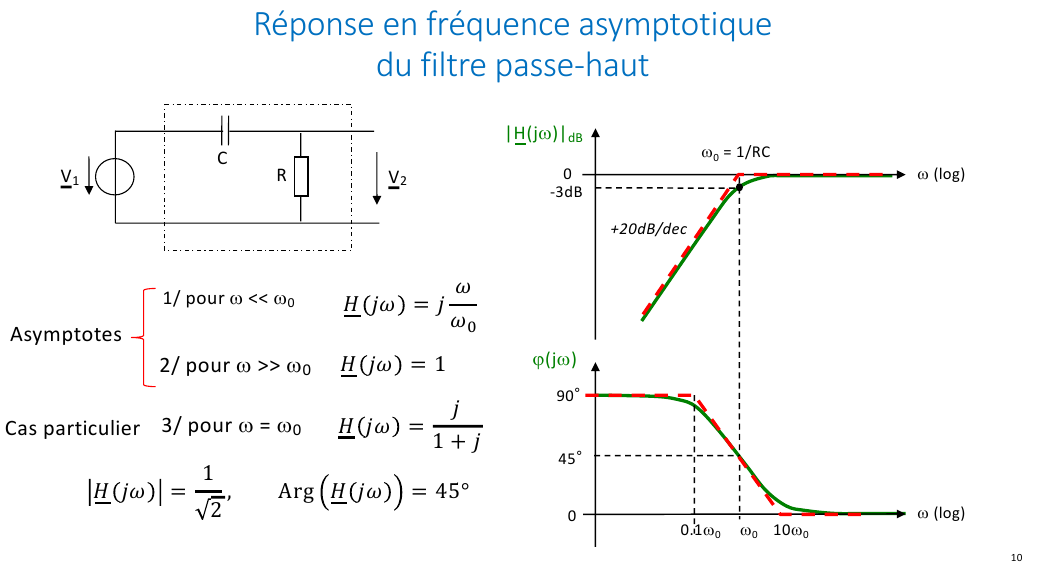
\includegraphics[
width=1.0\linewidth
]{../images/week06_10.png}

\end{center}


\begin{formula}

Asymptotes :

\begin{enumerate}[leftmargin=*,itemsep=1pt,topsep=1pt]

\item pour $\omega \ll \omega_0$ : $\underline{H}(j\omega) = j\frac{\omega}{\omega_0}$ ;

\item pour $\omega \gg \omega_0$ : $\underline{H}(j\omega) = 1$.

\end{enumerate}

Cas particulier, pour $\omega = \omega_0$ :

\[
\underline{H}(j\omega) = \frac{j}{1 + j}
\qquad
|\underline{H}(j\omega)| = \frac{1}{\sqrt 2}
\qquad
\operatorname{Arg}(\underline{H}(j\omega)) = 45°
\]

\end{formula}

Comme pour le passe-bas, le passe-haut peut être étudié de manière complète (courbe réelle) ou approximative avec les asymptotes. On obtient deux courbes aux caractéristiques similaires au cas précédent.


\begin{important}

\textbf{En très simple : le passe-bas à l'envers}

\textbf{Module} : à gauche, la courbe \textbf{monte} de $+20\,\text{dB}$ par décade (les graves sont très atténués) ; à partir de $\omega_0$, elle devient plate à $0\,\text{dB}$ (les aigus passent intacts).

\vspace{3pt}

\textbf{Phase} : elle part de $+90°$ (la sortie est en \textbf{avance} d'un quart de tour), passe par $+45°$ en $\omega_0$, et finit à $0°$.

\vspace{3pt}

\textbf{Comment trouver les asymptotes ?} On regarde qui \og gagne \fg{} dans $1 + j\frac{\omega}{\omega_0}$ :

\begin{itemize}

\item $\omega$ tout petit : le $1$ gagne, le bas vaut $\approx 1$, donc $\underline{H} \approx j\frac{\omega}{\omega_0}$ (une droite qui monte) ;

\item $\omega$ très grand : le $j\frac{\omega}{\omega_0}$ gagne, il se simplifie avec celui du haut, donc $\underline{H} \approx 1$ (plat à $0\,\text{dB}$).

\end{itemize}

\textbf{L'autre écriture} (avec $\omega_0/\omega$) donne la même chose, mais elle ne se découpe pas en briques : c'est pour ça qu'elle est difficile à exploiter.

\end{important}


%=========================================================
\section{Diagramme de Bode : module}


\begin{center}

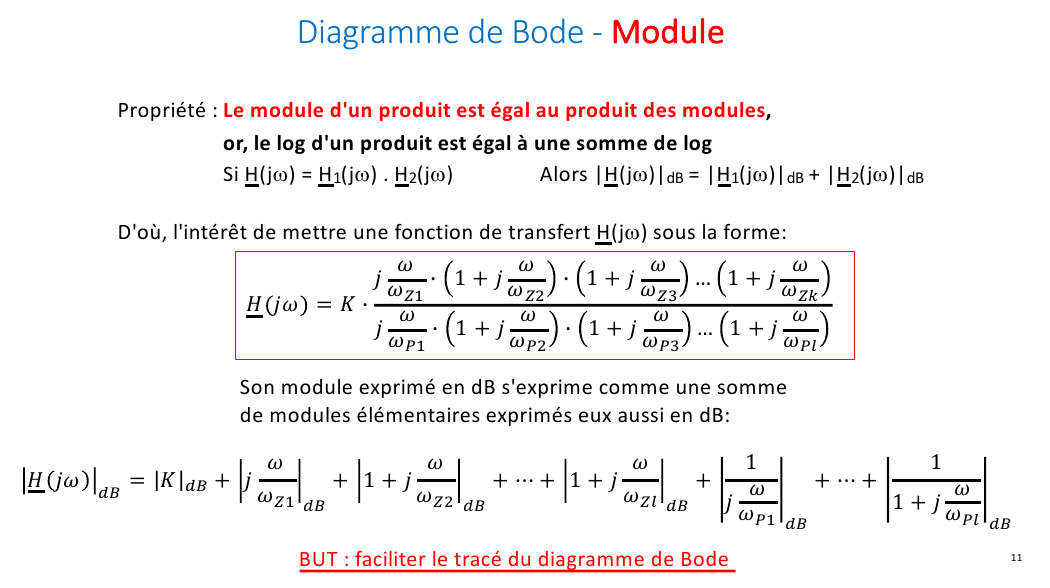
\includegraphics[
width=1.0\linewidth
]{../images/week06_11.png}

\end{center}

\textbf{Propriété :} le module d'un produit est égal au produit des modules, or le log d'un produit est égal à une somme de logs.


\begin{formula}

\[
\text{Si } \underline{H}(j\omega) = \underline{H}_1(j\omega)\cdot\underline{H}_2(j\omega)
\quad\text{alors}\quad
|\underline{H}(j\omega)|_{dB} = |\underline{H}_1(j\omega)|_{dB} + |\underline{H}_2(j\omega)|_{dB}
\]

D'où l'intérêt de mettre la fonction de transfert sous la forme canonique : son module en dB est une somme de modules élémentaires, eux aussi en dB :

\[
|\underline{H}(j\omega)|_{dB} = |K|_{dB} + \left|j\frac{\omega}{\omega_{Z1}}\right|_{dB} + \left|1 + j\frac{\omega}{\omega_{Z2}}\right|_{dB} + \cdots
\]
\[
\cdots + \left|\frac{1}{j\frac{\omega}{\omega_{P1}}}\right|_{dB} + \cdots + \left|\frac{1}{1 + j\frac{\omega}{\omega_{Pl}}}\right|_{dB}
\]

où :

\begin{itemize}

\item $\underline{H}_1$, $\underline{H}_2$ : deux morceaux (briques) de la fonction de transfert ;

\item $|\cdot|_{dB}$ : module en décibels [dB] ;

\item $\omega_{Zi}$, $\omega_{Pi}$ : pulsations des zéros et des pôles [rad/s].

\end{itemize}

\end{formula}

\textbf{But :} faciliter le tracé du diagramme de Bode. Le module d'un produit est égal au produit des modules, et le module d'un rapport est égal au rapport des modules. Le dessin du module complet est grandement facilité, car les modules de chaque terme de base donnent des allures très simples.


\begin{important}

\textbf{En très simple : la recette du module}

\begin{enumerate}[leftmargin=*,itemsep=1pt,topsep=1pt]

\item On écrit la fonction comme une multiplication de briques (forme canonique).

\item On dessine le module en dB de \textbf{chaque brique toute seule} (des segments de droite, voir les sections suivantes).

\item On \textbf{additionne} les dessins, intervalle par intervalle : à chaque fréquence, la hauteur totale = la somme des hauteurs de chaque brique.

\end{enumerate}

Ça marche grâce aux dB : multiplier les briques revient à additionner leurs dB. Les briques du bas (pôles) comptent en \textbf{négatif} : diviser, c'est soustraire en dB.

\end{important}


%=========================================================
\section{Module des fonctions élémentaires [1] : la constante $K$}


\begin{center}

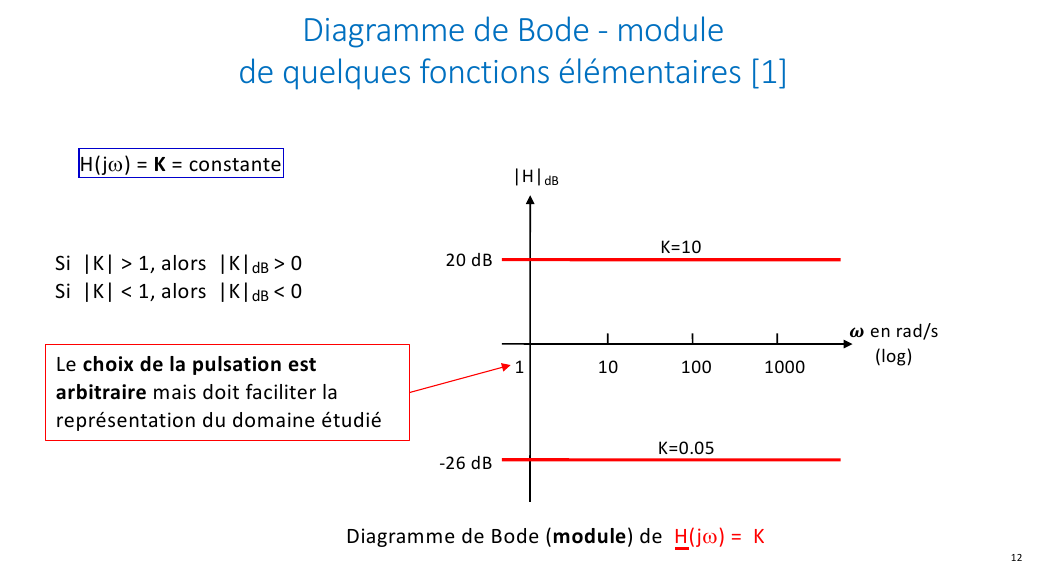
\includegraphics[
width=1.0\linewidth
]{../images/week06_12.png}

\end{center}


\begin{formula}

$\underline{H}(j\omega) = K$ = constante :

\begin{itemize}

\item si $|K| > 1$, alors $|K|_{dB} > 0$ ;

\item si $|K| < 1$, alors $|K|_{dB} < 0$.

\end{itemize}

\[
K = 10 \;\Rightarrow\; 20\log(10) = 20\,\text{dB}
\qquad
K = 0.05 \;\Rightarrow\; 20\log(0.05) \approx -26\,\text{dB}
\]

où $K$ : constante [sans unité] ; $\omega$ en [rad/s], sur une échelle logarithmique.

\end{formula}

Le choix de la pulsation de départ de l'axe est arbitraire, mais doit faciliter la représentation du domaine étudié. Le premier des cinq termes de base est une constante : si elle est supérieure à 1, le module est positif en dB, et négatif dans le cas contraire.


\begin{center}

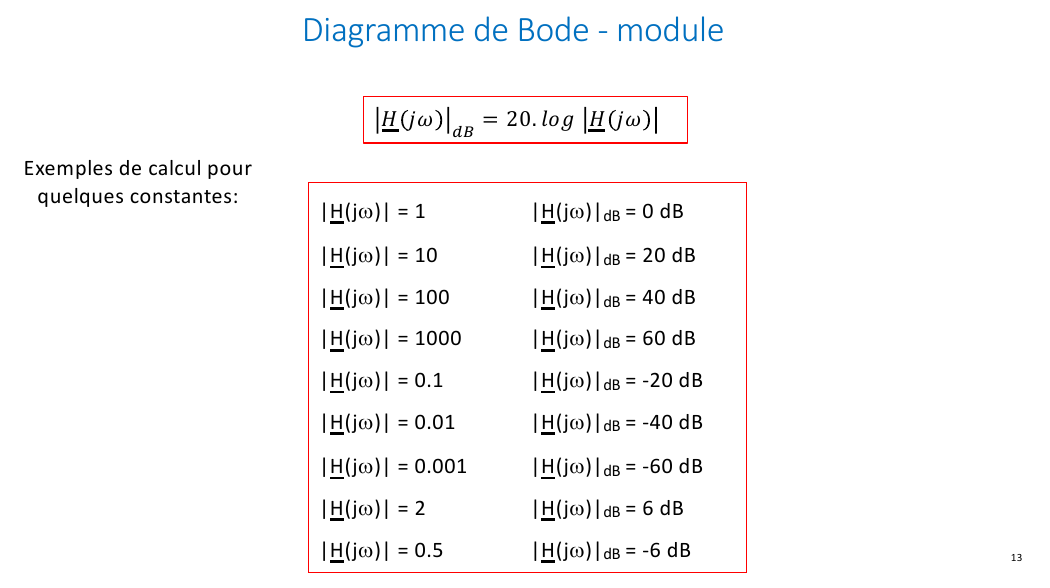
\includegraphics[
width=1.0\linewidth
]{../images/week06_13.png}

\end{center}


\begin{formula}

\[
|\underline{H}(j\omega)|_{dB} = 20\log|\underline{H}(j\omega)|
\]

\renewcommand{\arraystretch}{1.2}

\begin{center}

\begin{tabular}{|c|c||c|c|}

\hline

$|\underline{H}|$ & $|\underline{H}|_{dB}$ & $|\underline{H}|$ & $|\underline{H}|_{dB}$ \tabularnewline

\hline

$1$ & $0\,\text{dB}$ & $0.1$ & $-20\,\text{dB}$ \tabularnewline

$10$ & $20\,\text{dB}$ & $0.01$ & $-40\,\text{dB}$ \tabularnewline

$100$ & $40\,\text{dB}$ & $0.001$ & $-60\,\text{dB}$ \tabularnewline

$1000$ & $60\,\text{dB}$ & $0.5$ & $-6\,\text{dB}$ \tabularnewline

$2$ & $6\,\text{dB}$ & & \tabularnewline

\hline

\end{tabular}

\end{center}

\end{formula}

Ces quelques valeurs constantes particulières seront très utiles par la suite.


\begin{important}

\textbf{En très simple}

Une constante, c'est un circuit qui multiplie le signal par le même nombre $K$ à \textbf{toutes} les fréquences : son diagramme est une \textbf{ligne horizontale}, à la hauteur $20\log K$.

\begin{itemize}

\item $K$ plus grand que 1 (le circuit amplifie) : la ligne est au-dessus de $0\,\text{dB}$ ;

\item $K$ plus petit que 1 (le circuit atténue) : la ligne est en dessous.

\end{itemize}

\textbf{Le truc pour le tableau :} chaque zéro de plus derrière le 1 ajoute $20\,\text{dB}$ ($10 \rightarrow 20$, $100 \rightarrow 40$, $1000 \rightarrow 60$) ; chaque zéro après la virgule en enlève 20. Et doubler, c'est $+6\,\text{dB}$.

\end{important}


%=========================================================
\section{Module des fonctions élémentaires [2] : $j\frac{\omega}{\omega_Z}$ et $\frac{1}{j\omega/\omega_P}$}


\begin{center}

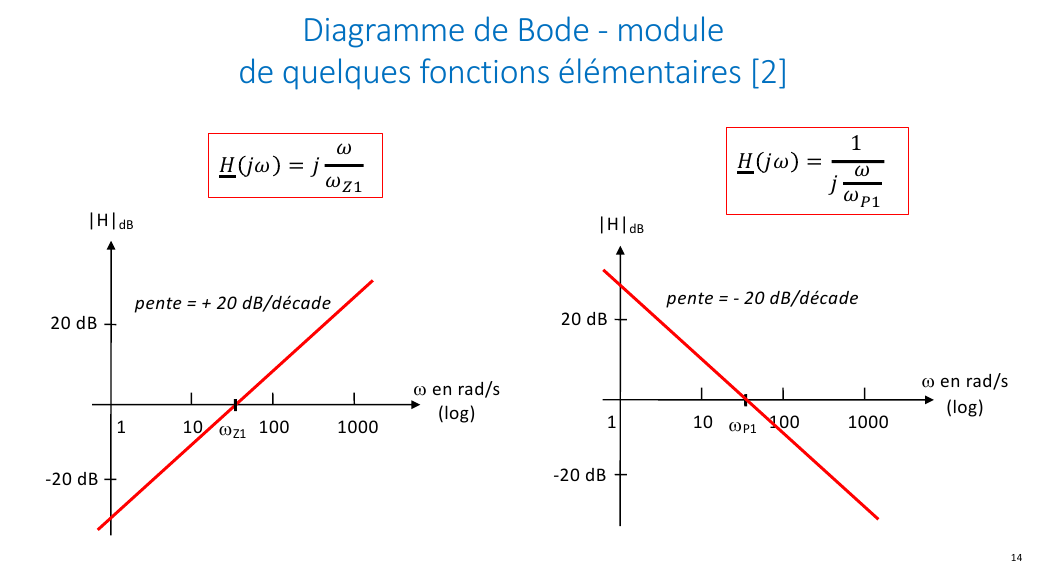
\includegraphics[
width=1.0\linewidth
]{../images/week06_14.png}

\end{center}


\begin{formula}

\[
\underline{H}(j\omega) = j\frac{\omega}{\omega_{Z1}}
\;\Rightarrow\;
|\underline{H}|_{dB} = 20\log\frac{\omega}{\omega_{Z1}}
\quad\text{pente} = +20\,\text{dB/décade}
\]
\[
\underline{H}(j\omega) = \frac{1}{j\frac{\omega}{\omega_{P1}}}
\;\Rightarrow\;
|\underline{H}|_{dB} = -20\log\frac{\omega}{\omega_{P1}}
\quad\text{pente} = -20\,\text{dB/décade}
\]

Les deux droites coupent l'axe des $0\,\text{dB}$ à leur pulsation caractéristique ($\omega_{Z1}$ ou $\omega_{P1}$).

où :

\begin{itemize}

\item $\omega_{Z1}$ : pulsation du zéro [rad/s] ; $\omega_{P1}$ : pulsation du pôle [rad/s] ;

\item $\omega$ : pulsation [rad/s], axe en échelle logarithmique.

\end{itemize}

\end{formula}

\textbf{Remarque importante :} travailler avec $a\log(X)$ sur une échelle logarithmique revient à travailler avec $a\,X$ sur une échelle linéaire. On peut donc représenter chaque dessin de manière linéaire, ce qui simplifie significativement la représentation globale (somme de dessins linéaires).

Le second terme est un imaginaire pur : il donne une pente constante de $+20\,\text{dB}$ par décade sur toute l'échelle des pulsations, qui coupe l'axe des $0\,\text{dB}$ à la pulsation caractéristique. Pour les pulsations inférieures, ce terme atténue le signal d'entrée ; pour les supérieures, il l'amplifie. Le troisième terme est symétrique du second : pente constante de $-20\,\text{dB}$ par décade, coupant aussi l'axe des $0\,\text{dB}$ à la pulsation caractéristique. Il atténue au-dessus et amplifie en dessous.


\begin{important}

\textbf{En très simple}

\textbf{La brique $j\frac{\omega}{\omega_Z}$} : sa taille vaut $\frac{\omega}{\omega_Z}$, donc elle grandit avec la fréquence. Quand la fréquence est multipliée par 10, la taille aussi, soit $+20\,\text{dB}$. Sur l'axe en échelle log, ça donne une \textbf{droite qui monte} de $20\,\text{dB}$ par décade.

\begin{itemize}

\item elle vaut $1$ (donc $0\,\text{dB}$) pile quand $\omega = \omega_Z$ : c'est là qu'elle croise l'axe ;

\item avant $\omega_Z$, elle est sous $0\,\text{dB}$ (elle rétrécit le signal) ; après, au-dessus (elle l'agrandit).

\end{itemize}

\textbf{La brique $\frac{1}{j\omega/\omega_P}$} : c'est l'inverse, une \textbf{droite qui descend} de $20\,\text{dB}$ par décade, qui croise aussi $0\,\text{dB}$ en $\omega_P$.

\vspace{3pt}

\textbf{Pourquoi une droite ?} Grâce à l'échelle log sur les deux axes (dB en haut, log en bas) : un \og $\log(\omega)$ \fg{} dessiné sur un axe en $\log(\omega)$, c'est une simple droite.

\end{important}


\begin{example}

$\omega_Z = 10\,\text{rad/s}$ : à $\omega = 1$ $\rightarrow$ $-20\,\text{dB}$ ; à $\omega = 10$ $\rightarrow$ $0\,\text{dB}$ ; à $\omega = 100$ $\rightarrow$ $+20\,\text{dB}$ ; à $\omega = 1000$ $\rightarrow$ $+40\,\text{dB}$.

\end{example}


%=========================================================
\section{Module des fonctions élémentaires [3] : $1 + j\frac{\omega}{\omega_Z}$ et son inverse}


\begin{center}

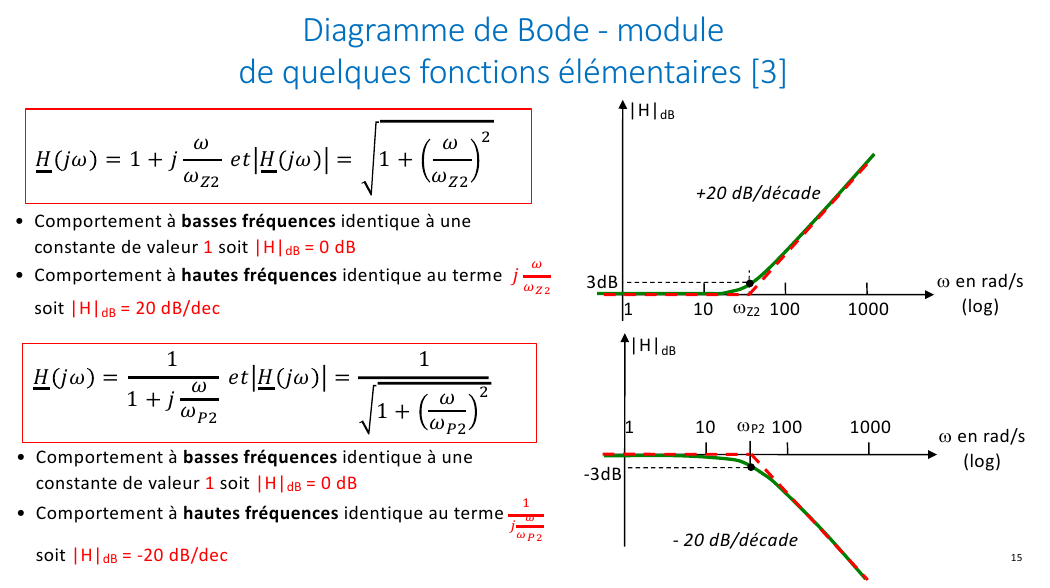
\includegraphics[
width=1.0\linewidth
]{../images/week06_15.png}

\end{center}


\begin{formula}

\[
\underline{H}(j\omega) = 1 + j\frac{\omega}{\omega_{Z2}}
\quad\text{et}\quad
|\underline{H}(j\omega)| = \sqrt{1 + \left(\frac{\omega}{\omega_{Z2}}\right)^2}
\]

\begin{itemize}

\item comportement à \textbf{basses fréquences} identique à une constante de valeur $1$, soit $|\underline{H}|_{dB} = 0\,\text{dB}$ ;

\item comportement à \textbf{hautes fréquences} identique au terme $j\frac{\omega}{\omega_{Z2}}$, soit $+20\,\text{dB/déc}$.

\end{itemize}

\[
\underline{H}(j\omega) = \frac{1}{1 + j\frac{\omega}{\omega_{P2}}}
\quad\text{et}\quad
|\underline{H}(j\omega)| = \frac{1}{\sqrt{1 + \left(\frac{\omega}{\omega_{P2}}\right)^2}}
\]

\begin{itemize}

\item comportement à \textbf{basses fréquences} identique à une constante de valeur $1$, soit $0\,\text{dB}$ ;

\item comportement à \textbf{hautes fréquences} identique au terme $\frac{1}{j\omega/\omega_{P2}}$, soit $-20\,\text{dB/déc}$.

\end{itemize}

Erreur maximale, à la pulsation caractéristique : $+3\,\text{dB}$ pour le zéro, $-3\,\text{dB}$ pour le pôle.

où $\omega_{Z2}$, $\omega_{P2}$ : pulsations caractéristiques [rad/s] ; $\omega$ [rad/s].

\end{formula}

Le quatrième terme ressemble au second, mais avec un $+1$ en plus : il a donc une partie réelle et une partie imaginaire. Son module met en évidence 2 asymptotes : une horizontale entre les basses pulsations et la pulsation caractéristique (pour $\omega \ll \omega_{Z}$, le terme $\omega/\omega_Z$ est négligeable devant 1), et une à $+20\,\text{dB/déc}$ au-delà (le $1$ est négligeable devant le terme imaginaire, et on retrouve le second terme). Les asymptotes approximent bien la réalité : l'erreur maximale est à la pulsation caractéristique et vaut $+3\,\text{dB}$. Le cinquième terme est le symétrique du quatrième, avec une erreur maximale de $-3\,\text{dB}$.


\begin{important}

\textbf{En très simple : le \og coude \fg{}}

Dans $1 + j\frac{\omega}{\omega_Z}$, il y a une bagarre entre le $1$ et le $j\frac{\omega}{\omega_Z}$ :

\begin{itemize}

\item \textbf{fréquence basse} : $\frac{\omega}{\omega_Z}$ est minuscule, le $1$ gagne. La brique vaut $\approx 1$, donc \textbf{plat à $0\,\text{dB}$} ;

\item \textbf{fréquence haute} : $\frac{\omega}{\omega_Z}$ est énorme, il gagne. La brique se comporte comme $j\frac{\omega}{\omega_Z}$ : \textbf{droite qui monte} de $20\,\text{dB/décade}$ ;

\item \textbf{pile en $\omega_Z$} : égalité, la brique vaut $1 + j$, de module $\sqrt{2}$, soit $+3\,\text{dB}$. C'est le seul endroit où le coude se trompe un peu.

\end{itemize}

Le dessin : plat jusqu'à $\omega_Z$, puis ça monte. Pour le pôle $\frac{1}{1 + j\omega/\omega_P}$, c'est pareil à l'envers : plat jusqu'à $\omega_P$, puis ça descend (c'est le passe-bas !).

\end{important}


%=========================================================
\section{Exemple de diagramme de Bode : module}


\begin{center}

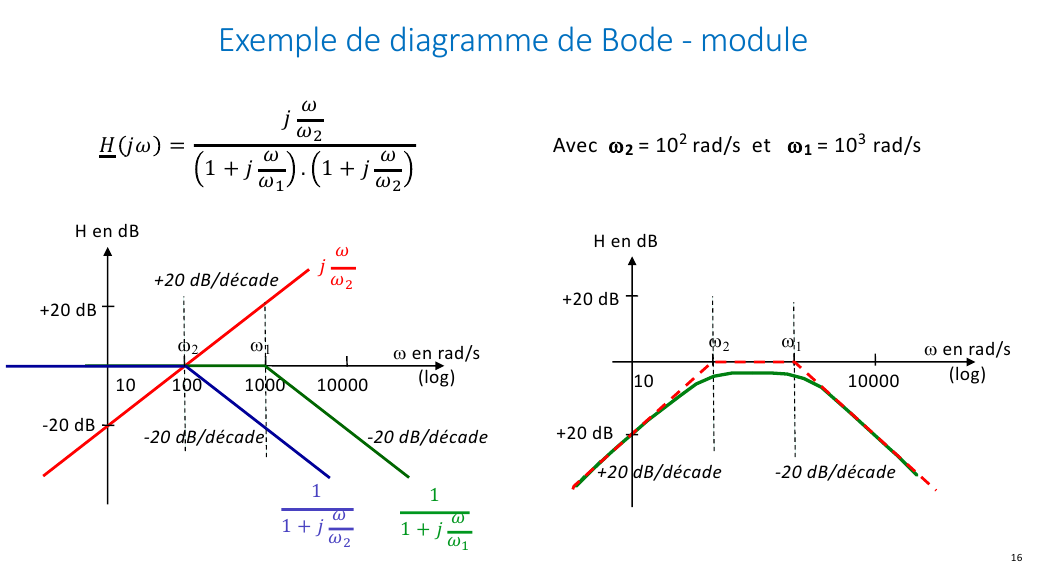
\includegraphics[
width=1.0\linewidth
]{../images/week06_16.png}

\end{center}


\begin{formula}

\[
\underline{H}(j\omega) = \frac{j\frac{\omega}{\omega_2}}{\left(1 + j\frac{\omega}{\omega_1}\right)\cdot\left(1 + j\frac{\omega}{\omega_2}\right)}
\quad\text{avec}\quad
\omega_2 = 10^2\,\text{rad/s},\ \omega_1 = 10^3\,\text{rad/s}
\]

\[
|\underline{H}|_{dB} = \left|j\frac{\omega}{\omega_2}\right|_{dB} + \left|\frac{1}{1 + j\frac{\omega}{\omega_2}}\right|_{dB} + \left|\frac{1}{1 + j\frac{\omega}{\omega_1}}\right|_{dB}
\]

où $\omega_1$, $\omega_2$ : pulsations caractéristiques [rad/s] ; $\omega$ [rad/s].

\end{formula}

Cette fonction de transfert met en évidence trois termes de base, chacun avec une allure propre et une pulsation caractéristique propre. Le dessin de chaque terme étant très simple, le dessin global demande très peu de travail, et le diagramme de Bode complet approxime bien la réalité.


\begin{important}

\textbf{En très simple : on empile les 3 briques (graphe de gauche)}

\begin{itemize}

\item \textbf{rouge} $j\frac{\omega}{\omega_2}$ : droite qui monte de $+20\,\text{dB/déc}$, qui croise $0\,\text{dB}$ en $\omega_2 = 100$ ;

\item \textbf{bleu} $\frac{1}{1 + j\omega/\omega_2}$ : plat à $0\,\text{dB}$ jusqu'à $100$, puis descend de $-20\,\text{dB/déc}$ ;

\item \textbf{vert} $\frac{1}{1 + j\omega/\omega_1}$ : plat à $0\,\text{dB}$ jusqu'à $1000$, puis descend de $-20\,\text{dB/déc}$.

\end{itemize}

\textbf{On additionne les pentes, zone par zone (graphe de droite)} :

\begin{itemize}

\item \textbf{avant 100} : seul le rouge bouge, $+20$ ; la courbe monte et arrive à $0\,\text{dB}$ en 100 ;

\item \textbf{entre 100 et 1000} : rouge $+20$, bleu $-20$, vert $0$ : total $0$, c'est \textbf{plat} à $0\,\text{dB}$ ;

\item \textbf{après 1000} : $+20 - 20 - 20 = -20\,\text{dB/déc}$, ça redescend.

\end{itemize}

\textbf{Résultat :} un \textbf{filtre passe-bande}. Il laisse passer les fréquences entre $100$ et $1000\,\text{rad/s}$ et atténue les autres.

\end{important}


%=========================================================
\section{Diagramme de Bode : argument ou phase}


\begin{center}

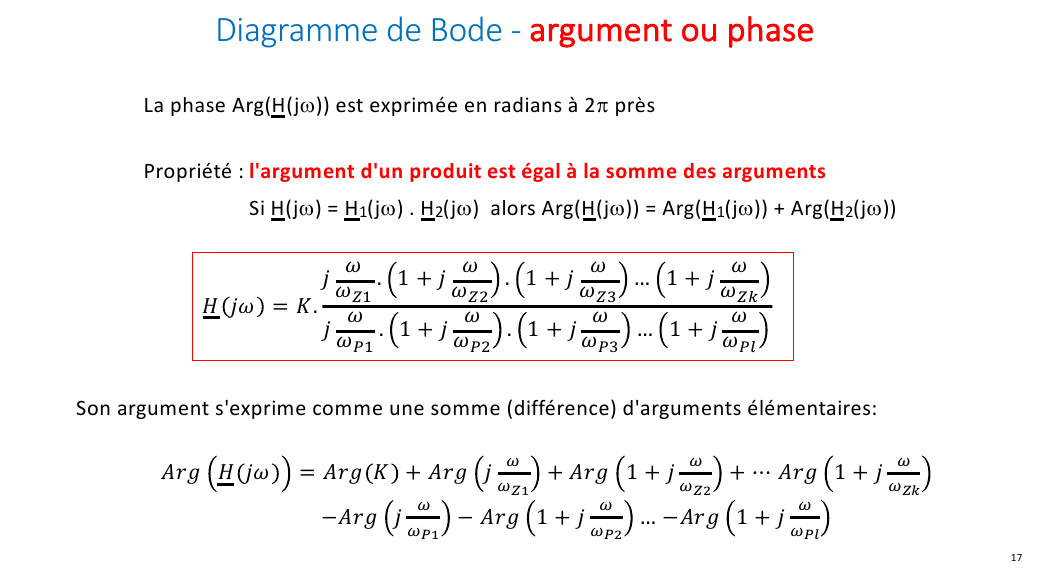
\includegraphics[
width=1.0\linewidth
]{../images/week06_17.png}

\end{center}

La phase $\operatorname{Arg}(\underline{H}(j\omega))$ est exprimée en radians, à $2\pi$ près.

\textbf{Propriété :} l'argument d'un produit est égal à la somme des arguments.


\begin{formula}

\[
\text{Si } \underline{H}(j\omega) = \underline{H}_1(j\omega)\cdot\underline{H}_2(j\omega)
\quad\text{alors}\quad
\operatorname{Arg}(\underline{H}(j\omega)) = \operatorname{Arg}(\underline{H}_1(j\omega)) + \operatorname{Arg}(\underline{H}_2(j\omega))
\]

Pour la forme canonique, l'argument est une somme (différence) d'arguments élémentaires :

\[
\operatorname{Arg}(\underline{H}(j\omega)) = \operatorname{Arg}(K) + \operatorname{Arg}\left(j\frac{\omega}{\omega_{Z1}}\right) + \operatorname{Arg}\left(1 + j\frac{\omega}{\omega_{Z2}}\right) + \cdots
\]
\[
\cdots - \operatorname{Arg}\left(j\frac{\omega}{\omega_{P1}}\right) - \operatorname{Arg}\left(1 + j\frac{\omega}{\omega_{P2}}\right) - \cdots
\]

où :

\begin{itemize}

\item $\operatorname{Arg}$ : argument, la phase [rad] ou [°] ;

\item les termes du numérateur (zéros) s'ajoutent, ceux du dénominateur (pôles) se soustraient.

\end{itemize}

\end{formula}

L'argument d'un produit est égal à la somme des arguments, et l'argument d'un rapport à la différence des arguments. Comme pour le module, le dessin de la phase complète est facilité.


\begin{important}

\textbf{En très simple}

Pour la phase, pas besoin de décibels : les angles s'additionnent déjà tout seuls quand on multiplie des complexes (semaine 05 : multiplier, c'est tourner d'un angle puis d'un autre).

\vspace{3pt}

Même recette que pour le module :

\begin{enumerate}[leftmargin=*,itemsep=1pt,topsep=1pt]

\item dessiner la phase de chaque brique toute seule ;

\item additionner les briques du haut, soustraire celles du bas ;

\item additionner les dessins, zone par zone.

\end{enumerate}

\end{important}


%=========================================================
\section{Phase des fonctions élémentaires [1] et [2] : $K$, $j\frac{\omega}{\omega_Z}$, $\frac{1}{j\omega/\omega_P}$}


\begin{center}

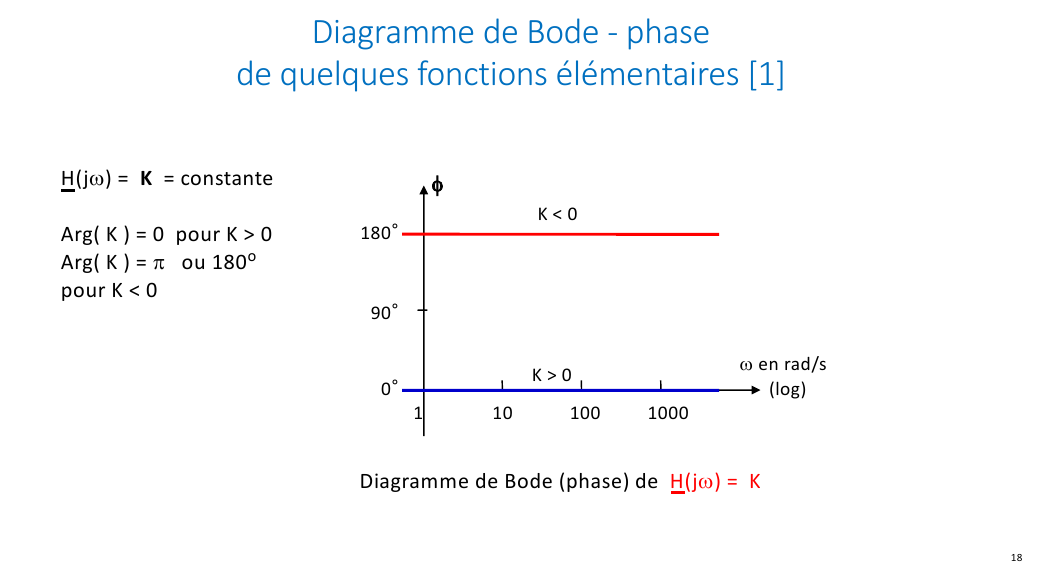
\includegraphics[
width=1.0\linewidth
]{../images/week06_18.png}

\end{center}


\begin{formula}

$\underline{H}(j\omega) = K$ = constante :

\[
\operatorname{Arg}(K) = 0 \ \text{pour}\ K > 0
\qquad
\operatorname{Arg}(K) = \pi \ (180°) \ \text{pour}\ K < 0
\]

\end{formula}

Pour les termes constants, selon qu'ils sont positifs ou négatifs, l'argument donne deux déphasages possibles : $0$ ou $\pi$. Pour les modules, le signe n'intervenait pas : seule la valeur absolue comptait.


\begin{center}

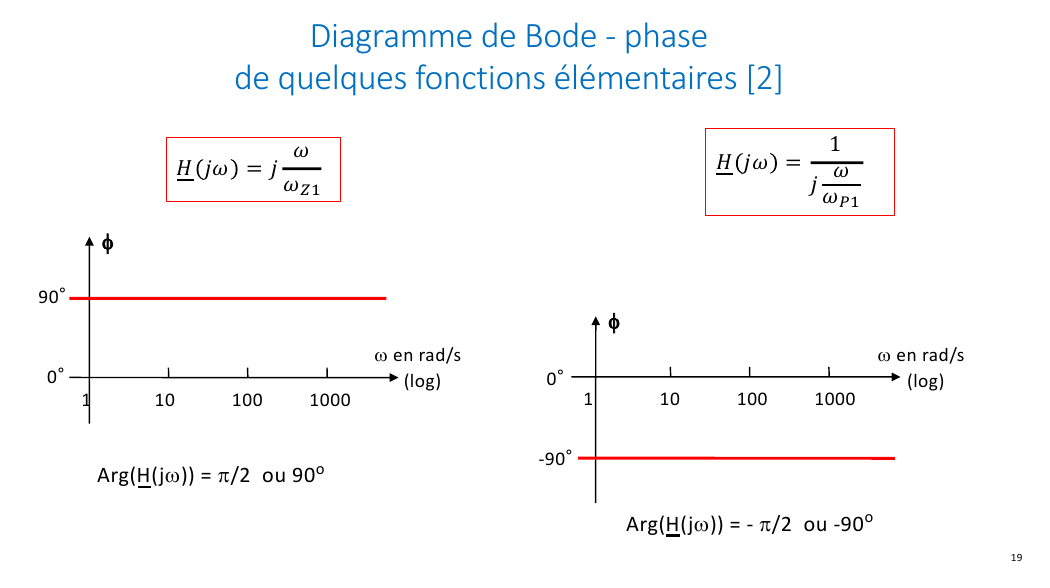
\includegraphics[
width=1.0\linewidth
]{../images/week06_19.png}

\end{center}


\begin{formula}

\[
\underline{H}(j\omega) = j\frac{\omega}{\omega_{Z1}}
\;\Rightarrow\;
\operatorname{Arg}(\underline{H}(j\omega)) = \frac{\pi}{2} \ \text{ou}\ 90°
\]
\[
\underline{H}(j\omega) = \frac{1}{j\frac{\omega}{\omega_{P1}}}
\;\Rightarrow\;
\operatorname{Arg}(\underline{H}(j\omega)) = -\frac{\pi}{2} \ \text{ou}\ -90°
\]

où $K$ : constante ; $\omega_{Z1}$, $\omega_{P1}$ : pulsations caractéristiques [rad/s] ; la phase en [rad] ou [°].

\end{formula}

Le second terme donne un déphasage constant de $90°$ : c'est un imaginaire pur, la partie réelle n'existe pas, et l'arctg$(Y/0)$ vaut toujours $90°$. Le troisième terme est le symétrique du second : un déphasage constant de $-90°$.


\begin{important}

\textbf{En très simple : trois lignes horizontales}

\begin{itemize}

\item \textbf{$K$ positif} : un nombre positif est sur l'axe réel, vers la droite : angle $0$. Le signal n'est pas décalé.

\item \textbf{$K$ négatif} : il pointe vers la gauche : angle $180°$. Le signal est \textbf{retourné} (les bosses deviennent des creux).

\item \textbf{$j\frac{\omega}{\omega_Z}$} : un nombre avec juste un $j$ pointe tout droit vers le haut : $+90°$, à toutes les fréquences (sa taille change, sa direction jamais).

\item \textbf{$\frac{1}{j\omega/\omega_P}$} : diviser par $j$, c'est tourner d'un quart de tour en arrière : $-90°$, à toutes les fréquences.

\end{itemize}

Ces trois briques ont une phase \textbf{constante} : des lignes horizontales sur le diagramme.

\end{important}


%=========================================================
\section{Phase des fonctions élémentaires [3] : $1 + j\frac{\omega}{\omega_Z}$ et son inverse}


\begin{center}

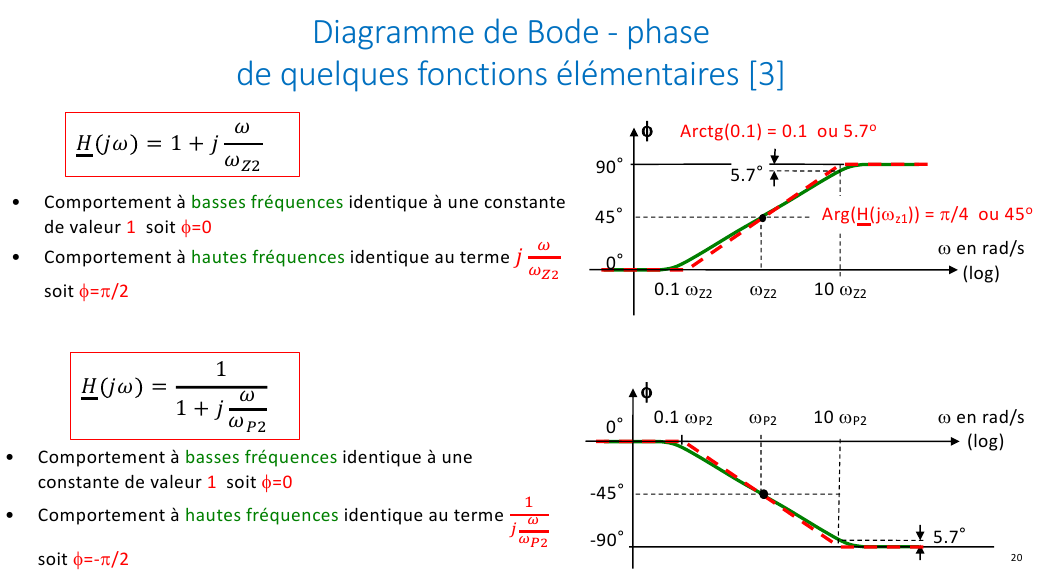
\includegraphics[
width=1.0\linewidth
]{../images/week06_20.png}

\end{center}


\begin{formula}

\[
\underline{H}(j\omega) = 1 + j\frac{\omega}{\omega_{Z2}}
\;\Rightarrow\;
\operatorname{Arg} = \operatorname{arctg}\frac{\omega}{\omega_{Z2}}
\]

\begin{itemize}

\item basses fréquences : identique à une constante de valeur $1$, soit $\phi = 0$ ;

\item hautes fréquences : identique au terme $j\frac{\omega}{\omega_{Z2}}$, soit $\phi = \pi/2$ ;

\item en $\omega_{Z2}$ : $\operatorname{Arg}(\underline{H}(j\omega_{Z2})) = \pi/4$ ou $45°$ ;

\item en $0.1\,\omega_{Z2}$ : $\operatorname{arctg}(0.1) = 0.1$ rad, soit $5.7°$ (écart avec l'asymptote).

\end{itemize}

\[
\underline{H}(j\omega) = \frac{1}{1 + j\frac{\omega}{\omega_{P2}}}
\;\Rightarrow\;
\operatorname{Arg} = -\operatorname{arctg}\frac{\omega}{\omega_{P2}}
\]

\begin{itemize}

\item basses fréquences : constante de valeur $1$, soit $\phi = 0$ ;

\item hautes fréquences : identique au terme $\frac{1}{j\omega/\omega_{P2}}$, soit $\phi = -\pi/2$ ;

\item en $\omega_{P2}$ : $-45°$.

\end{itemize}

où $\phi$ : phase [rad] ou [°] ; $\omega_{Z2}$, $\omega_{P2}$ : pulsations caractéristiques [rad/s].

\end{formula}

Le quatrième terme a une partie réelle et une partie imaginaire. Son allure se décompose en trois zones : les basses pulsations jusqu'à $0.1\,\omega_{Z}$ donnent un déphasage nul ; de $10\,\omega_{Z}$ aux hautes pulsations, un déphasage de $90°$ ; la zone intermédiaire rejoint les deux asymptotes, avec $45°$ à la pulsation caractéristique. L'erreur maximale entre la courbe réelle et l'asymptotique vaut $5.7°$, aux deux pulsations $0.1\,\omega_Z$ et $10\,\omega_Z$. Le cinquième terme est le symétrique du quatrième : asymptote à $-90°$ et $-45°$ à la pulsation caractéristique, avec la même erreur maximale de $5.7°$ en valeur absolue.


\begin{important}

\textbf{En très simple : la rampe sur deux décades}

Même bagarre que pour le module entre le $1$ et le $j\frac{\omega}{\omega_Z}$ :

\begin{itemize}

\item \textbf{fréquence basse} : le $1$ gagne, le nombre pointe vers la droite : $0°$ ;

\item \textbf{fréquence haute} : le $j\frac{\omega}{\omega_Z}$ gagne, il pointe vers le haut : $90°$ ;

\item \textbf{pile en $\omega_Z$} : $1 + j$, pile entre les deux : $45°$.

\end{itemize}

\textbf{Le dessin à la règle} : plat à $0°$ jusqu'à $\frac{\omega_Z}{10}$, plat à $90°$ à partir de $10\,\omega_Z$, et entre les deux une \textbf{rampe droite} qui monte de $90°$ en deux décades (donc $45°$ par décade) et passe par $45°$ en $\omega_Z$.

\vspace{3pt}

\textbf{Attention, différence avec le module :} le coude du module est en $\omega_Z$, mais la rampe de la phase commence une décade \textbf{avant} et finit une décade \textbf{après}. Pour le pôle, même chose vers le bas : de $0°$ à $-90°$.

\end{important}


%=========================================================
\section{Exemple de diagramme de Bode : phase}


\begin{center}

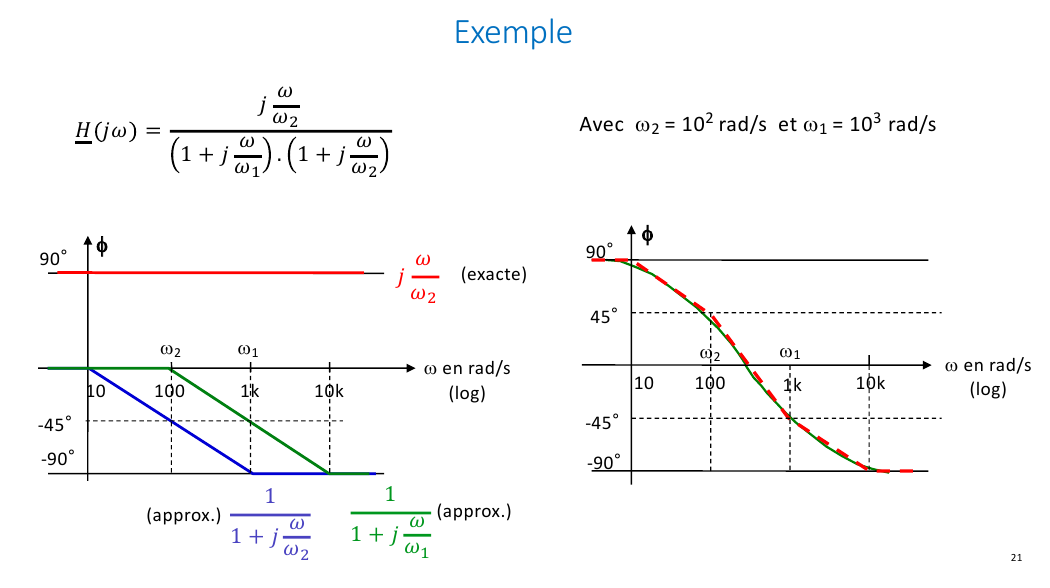
\includegraphics[
width=1.0\linewidth
]{../images/week06_21.png}

\end{center}


\begin{formula}

Même fonction de transfert que pour l'exemple du module :

\[
\underline{H}(j\omega) = \frac{j\frac{\omega}{\omega_2}}{\left(1 + j\frac{\omega}{\omega_1}\right)\cdot\left(1 + j\frac{\omega}{\omega_2}\right)}
\quad\text{avec}\quad
\omega_2 = 10^2\,\text{rad/s},\ \omega_1 = 10^3\,\text{rad/s}
\]

\[
\operatorname{Arg}(\underline{H}) = \operatorname{Arg}\left(j\frac{\omega}{\omega_2}\right) - \operatorname{Arg}\left(1 + j\frac{\omega}{\omega_2}\right) - \operatorname{Arg}\left(1 + j\frac{\omega}{\omega_1}\right)
\]

où $\omega_1$, $\omega_2$ : pulsations caractéristiques [rad/s] ; la phase en [°].

\end{formula}

On reprend la même fonction de transfert que pour le diagramme de Bode en module, chaque terme ayant une allure propre. Le dessin de chaque terme est à peine plus complexe, le dessin global demande un peu plus de subtilité, et le diagramme complet approxime toujours aussi bien la réalité.


\begin{important}

\textbf{En très simple : on empile les 3 briques (graphe de gauche)}

\begin{itemize}

\item \textbf{rouge} $j\frac{\omega}{\omega_2}$ : $+90°$ partout (exact) ;

\item \textbf{bleu} $\frac{1}{1 + j\omega/\omega_2}$ : $0°$ jusqu'à $10$, rampe jusqu'à $-90°$ atteint en $1000$ ($-45°$ en $100$) ;

\item \textbf{vert} $\frac{1}{1 + j\omega/\omega_1}$ : $0°$ jusqu'à $100$, rampe jusqu'à $-90°$ atteint en $10\,000$ ($-45°$ en $1000$).

\end{itemize}

\textbf{On additionne, point par point (graphe de droite)} :

\begin{itemize}

\item avant $10$ : $90 + 0 + 0 = 90°$ ;

\item en $100$ : $90 - 45 - 0 = 45°$ ;

\item en $1000$ : $90 - 90 - 45 = -45°$ ;

\item après $10\,000$ : $90 - 90 - 90 = -90°$.

\end{itemize}

On relie ces points par des segments : la phase descend de $+90°$ à $-90°$. Dans la bande qui passe (entre $100$ et $1000$), elle traverse $0°$ : c'est là que la sortie est le moins décalée.

\end{important}


\end{multicols}

\end{document}
